\chapter{Theoretical Framework}
\label{ch:theoretical_framework}

The development of continuous neurocognitive assessment systems is grounded in the convergence of neurophysiological principles, precision electronic engineering, and computer science. This chapter systematizes the critical concepts required for understanding the proposed architecture, addressing the stochastic nature of biological signals, the electrophysiological manifestations of Attention-Deficit/Hyperactivity Disorder (ADHD), the principles of low-noise acquisition architectures, and the challenges inherent to temporal synchronization in heterogeneous digital systems.

\section{Neurophysiology and Event-Related Potentials (ERPs)}
\label{sec:neurophysiology}

Electroencephalography (EEG) constitutes a non-invasive technique for recording cerebral bioelectric activity via transducers arranged on the scalp. While continuous EEG analysis allows for the monitoring of basal brain states—such as wakefulness, sleep, or convulsive pathologies—cognitive neuroscience research requires isolating specific neuronal responses associated with sensory, motor, or cognitive stimuli. These voltage fluctuations, known as Event-Related Potentials (ERPs), represent the synchronized activity of pyramidal neuronal populations in response to information processing.

\begin{figure}[ht]
    \centering
    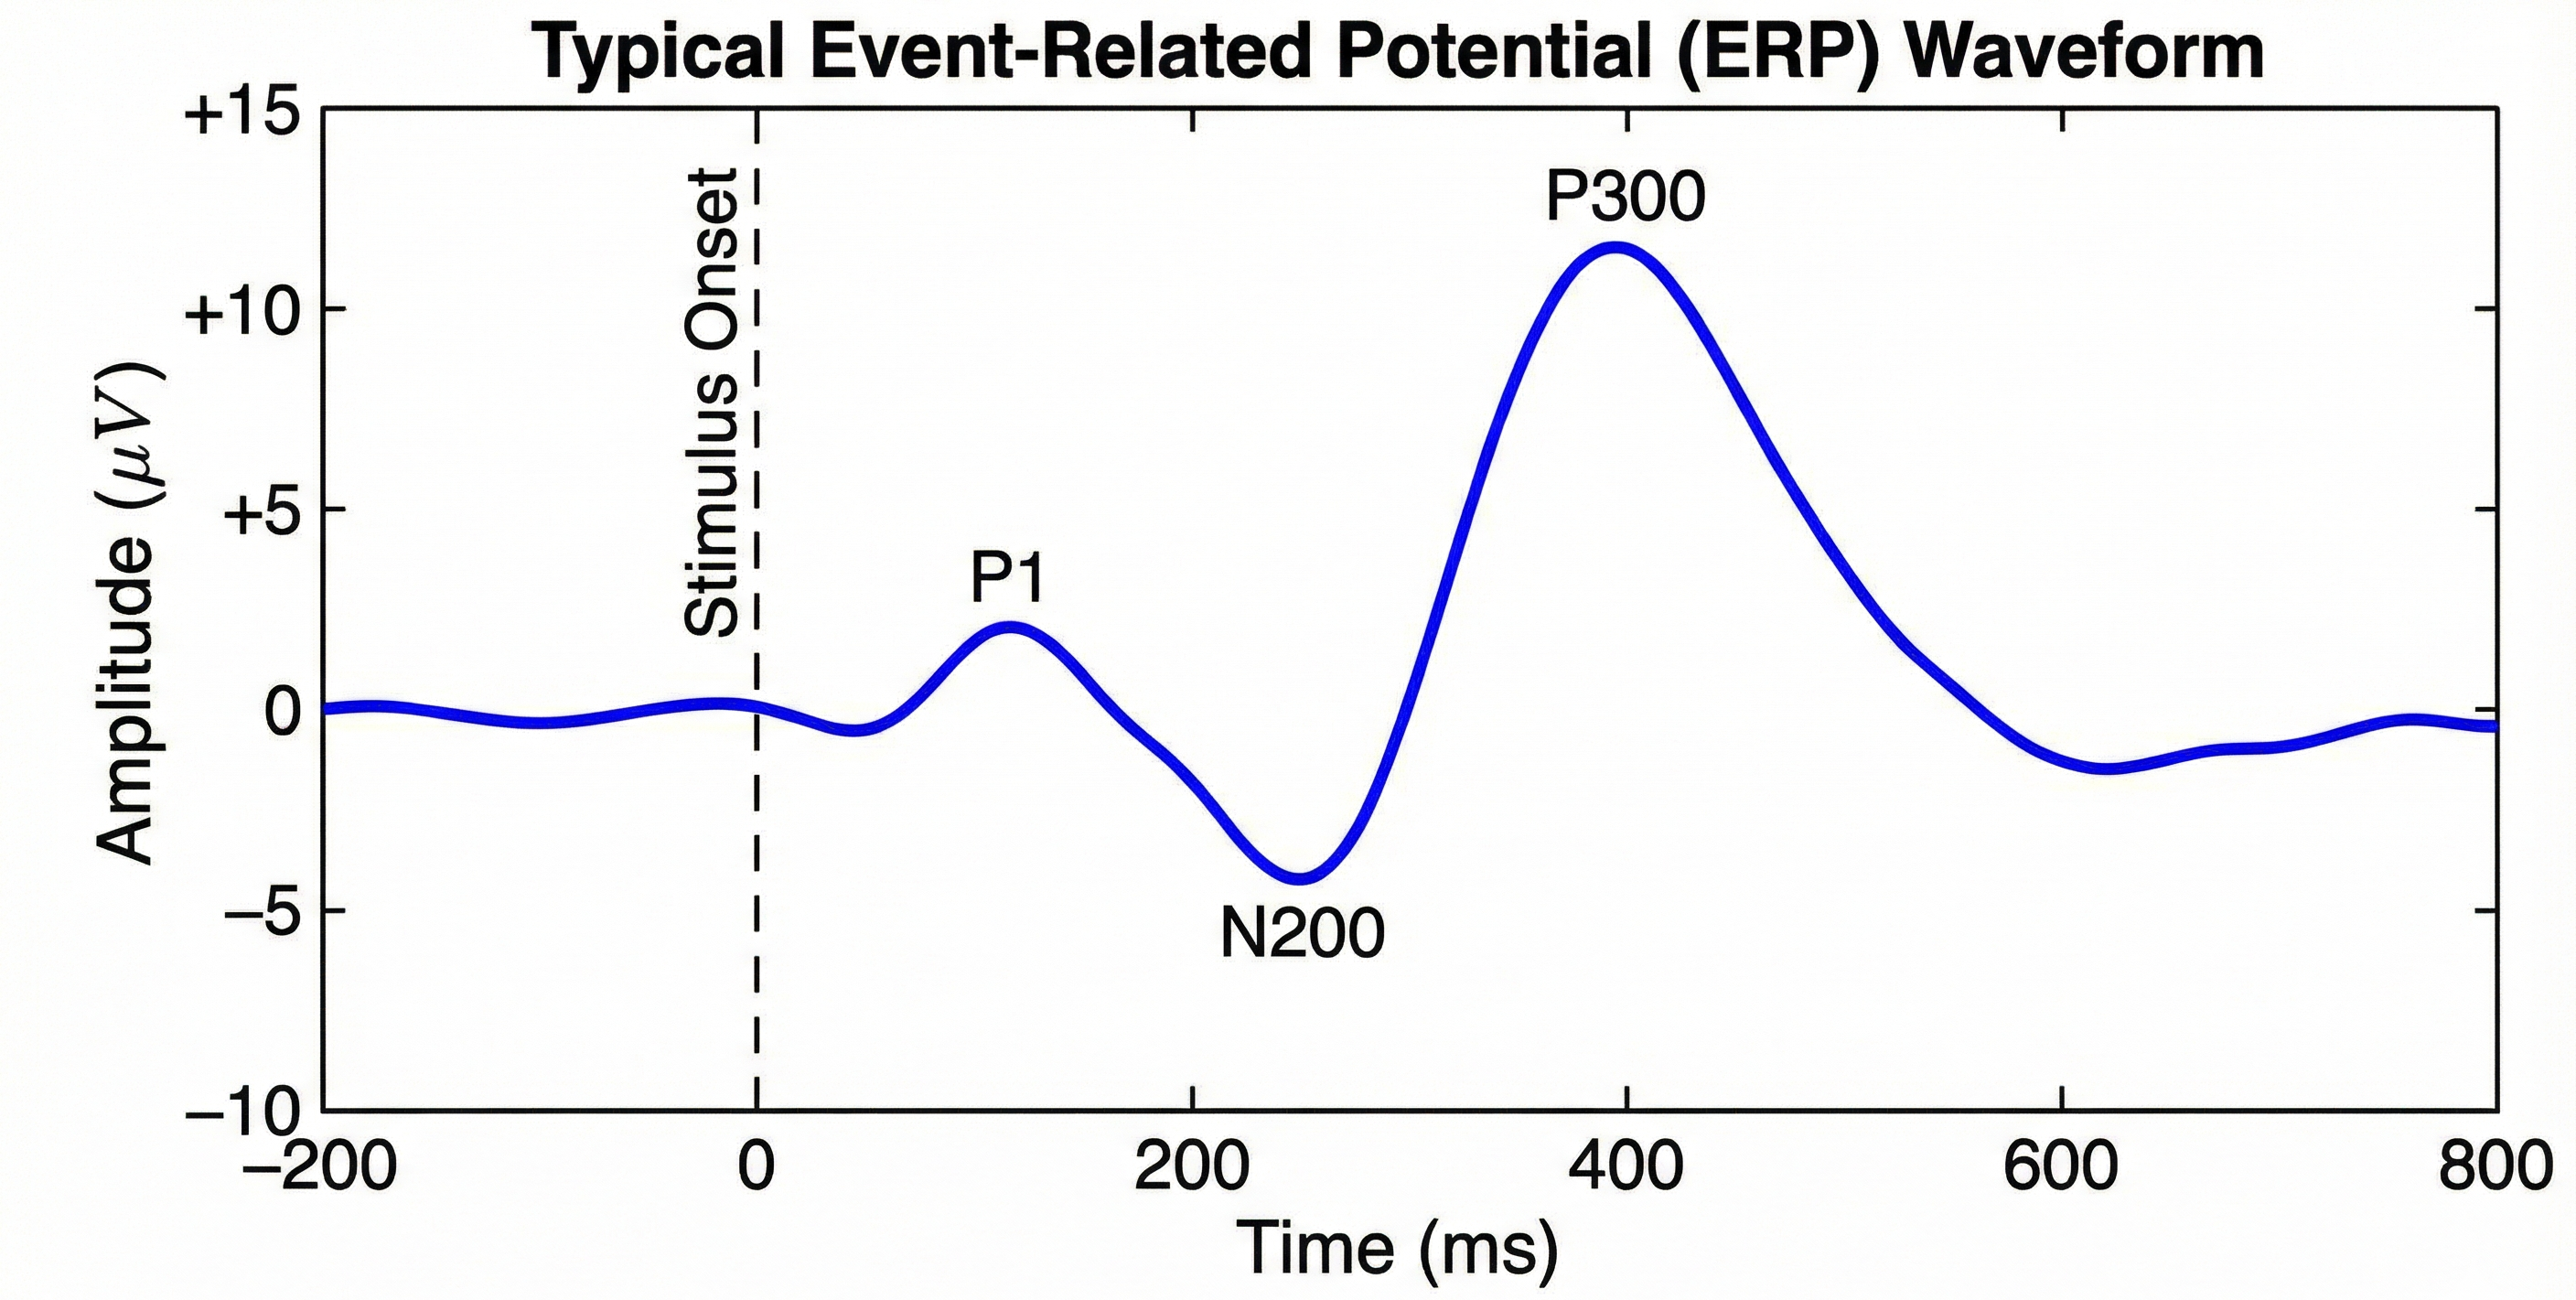
\includegraphics[width=0.8\textwidth]{Cap_2/Figure/p300_waveform.png}
    \caption{Characteristic morphology of an Event-Related Potential (ERP), highlighting exogenous and endogenous components such as the N200 and P300.}
    \label{fig:p300_waveform}
\end{figure}

Within the complex morphology of ERPs, two endogenous components are of particular interest for neurocognitive evaluation and the implementation of serious games in the context of this project. The first is the N200 (or N2) component, a negative deflection that reaches its maximum amplitude between 200 and 350 ms post-stimulus. This component is functionally linked to executive control, specifically in mismatch detection processes and the inhibition of motor responses. The second component, the P300 (or P3b), manifests as a prominent positive deflection with a latency of 300 to 600 ms. Its amplitude is modulated by the allocation of attentional resources and the updating of working memory, being particularly sensitive to stimulus improbability (the \textit{oddball} paradigm). Due to these characteristics, the P300 is consolidated as a robust biomarker for quantifying cognitive load and attentional deficits.

The detection of these components presents a significant challenge in signal processing due to their low signal-to-noise ratio (SNR). ERPs possess typical amplitudes in the range of $1\mu V$ to $20\mu V$, frequently remaining masked by background EEG activity, the magnitude of which oscillates between $50\mu V$ and $100\mu V$. To extract the signal of interest, the technique of coherent signal averaging is employed. Assuming that background noise is a stochastic process with zero mean and is uncorrelated with the stimulus, by averaging $N$ trials, the noise amplitude decreases in proportion to $1/\sqrt{N}$, while the ERP signal remains constant.

However, the validity of this technique depends strictly on temporal stability. Variability in the synchronization marker's latency, a phenomenon termed \textit{jitter}, introduces systematic errors in the resulting average. Mathematically, if the trigger latency follows a normal distribution with standard deviation $\sigma_t$, the averaging process acts as a low-pass filter on the original waveform, attenuating high-frequency components and distorting peak amplitude. A jitter greater than 10 ms ($\sigma_t > 10$ ms) is sufficient to degrade the morphology of the N200 component, compromising the diagnostic utility of the data. Consequently, acquisition systems must guarantee strict real-time (\textit{hard real-time}) synchronization to preserve the spectral and temporal integrity of the biomarkers.

\section{Electrophysiological Manifestations of ADHD}
\label{sec:adhd_manifestations}

Attention-Deficit/Hyperactivity Disorder (ADHD) is a neurodevelopmental condition characterized by persistent patterns of inattention, hyperactivity, and impulsivity. Clinically, the diagnosis of ADHD relies heavily on behavioral observations and subjective rating scales. However, electrophysiological techniques offer objective biomarkers that reflect the underlying neurological atypicalities associated with the disorder.

In resting-state EEG, individuals with ADHD frequently exhibit an elevated Theta/Beta ratio (TBR) compared to neurotypical peers. This ratio reflects an excess of slow-wave (Theta) activity, often associated with cortical underarousal or drowsiness, and a deficit in fast-wave (Beta) activity, which is linked to active concentration and cognitive engagement. While the TBR has been extensively studied as a potential diagnostic metric, its clinical utility is complemented by the analysis of dynamic brain responses during cognitive tasks.

During cognitive paradigms, such as continuous performance tests (CPTs) or the \textit{oddball} task, ERPs provide a window into the temporal dynamics of information processing in ADHD. The most consistent finding is a reduction in the amplitude of the P300 component. This attenuation is theorized to reflect deficits in the allocation of attentional resources and the updating of context in working memory. Furthermore, abnormalities in the N200 component are frequently observed, particularly during tasks requiring inhibitory control (e.g., Go/No-Go tasks). A reduced N200 amplitude in these contexts suggests difficulties in conflict monitoring and the suppression of prepotent motor responses, aligning with the impulsivity characteristic of the disorder.

Continuous EEG monitoring coupled with interactive tasks (like serious games) aims to systematically elicit and quantify these electrophysiological markers, providing a quantitative basis for assessing cognitive performance and the efficacy of therapeutic interventions in ADHD.

\section{Principles of Mixed-Signal Embedded Hardware Design}
\label{sec:hardware_principles}

The fidelity in the digitization of biopotentials is determined by the topology of the Analog Front-End (AFE). Modern acquisition architectures integrate specific analog-to-digital converters (ADCs) designed for biomedical instrumentation, which typically implement a Delta-Sigma ($\Delta\Sigma$) modulation architecture rather than traditional Successive Approximation Register (SAR) converters.

The $\Delta\Sigma$ architecture offers superior advantages in terms of dynamic range and noise rejection through two main mechanisms: oversampling and noise shaping. The device samples the input signal at a modulation frequency ($f_{mod}$) significantly higher than the Nyquist rate, distributing quantization noise power over a wider spectrum. Subsequently, the modulator shifts this noise toward high frequencies, outside the biological band of interest (0--100 Hz), allowing a digital decimation filter to eliminate it effectively while reducing the data rate to the output frequency configured by the user.

\begin{figure}[ht]
    \centering
    \includegraphics[width=0.8\textwidth]{Cap_2/Figure/delta_sigma_block.png}
    \caption{Simplified functional scheme of the modulation and filtering stage in a Delta-Sigma architecture ADC.}
    \label{fig:delta_sigma}
\end{figure}

A critical aspect for functional connectivity and EEG coherence analysis is sampling simultaneity. In older multiplexed systems, a single ADC core switches sequentially between channels, introducing a systematic phase delay ($t_{skew}$) between electrodes. Modern biomedical ADCs mitigate this problem by incorporating independent $\Delta\Sigma$ modulators for each channel, guaranteeing a virtually null $t_{skew}$ and preserving the real phase relationship between different cortical regions.

To manage data flow without sacrificing temporal determinism, advanced acquisition designs adopt a heterogeneous computing architecture that decouples acquisition from high-level processing. This structure typically comprises a Microcontroller Unit (MCU) operating in real-time, coupled with a Microprocessor Unit (MPU) for complex application tasks. The MCU operates under strict real-time constraints (either on \textit{bare-metal} or with a lightweight RTOS), reacting to ADC hardware interrupts on microsecond scales to capture and timestamp samples without buffer overflows. Meanwhile, the MPU manages computationally intensive and non-deterministic tasks, such as protocol stacks and file system storage. This division of responsibilities isolates bio-signal acquisition from the variable latencies introduced by high-level operating system schedulers, ensuring data temporal integrity.

\section{Principles of Data Synchronization}
\label{sec:sync_principles}

Precise synchronization between physiological recordings and external events (such as visual/auditory stimuli in a game) constitutes a central technical challenge in BCI and neurocognitive assessment systems. The selection of a synchronization method implies a trade-off between temporal precision, implementation complexity, and intrusion into the user experience. Table \ref{tab:sync_methods} summarizes the characteristics of the predominant approaches.

\begin{table}[ht]
    \centering
    \caption{Comparative analysis of synchronization methods for BCI systems.}
    \label{tab:sync_methods}
    \begin{tabular}{p{3cm} p{5cm} p{2.5cm} p{3.5cm}}
        \toprule
        \textbf{Method}        & \textbf{Mechanism}                                                         & \textbf{Precision}  & \textbf{Implementation}                \\
        \midrule
        Optical (Photodiode)   & Physical detection of screen luminance changes by an external sensor.      & High ($<1$ ms)      & High (Additional hardware required).   \\
        Network (LSL)          & Synchronization via local network protocol and software jitter correction. & Medium ($<5$ ms)    & Low (Software only).                   \\
        Hardware Trigger (TTL) & Direct electrical signal from Parallel/USB port to the ADC.                & Very High ($<1$ ms) & Medium (Requires specific interfaces). \\
        \bottomrule
    \end{tabular}
\end{table}

There are contrasting approaches to addressing this problem. Optical synchronization, based on photodiodes attached to the monitor, is considered the ``gold standard'' for validation, as it detects the physical change of pixels, bypassing software, operating system, and GPU rendering latencies. However, its requirement for external hardware limits its viability in massive clinical deployments. As a scalable alternative, the \textit{Lab Streaming Layer} (LSL) protocol offers a middleware solution that unifies disparate data streams by assigning timestamps referenced to a common clock and drift correction algorithms. While LSL simplifies integration, its final accuracy remains dependent on local network stability and the stimulation engine's ability to report the event time accurately.

In customized physical interfaces, standard buses like USB introduce non-trivial latency considerations, especially for the transmission of marking commands (\textit{soft-triggers}) from a PC or tablet to an amplifier. As a host-controlled bus utilizing polling, data transfer is discretized into frame intervals (1 ms in \textit{Full Speed}) or microframes ($125 \mu s$ in \textit{High Speed}). Additionally, data traverses the operating system driver stack, where it may be stored in intermediate buffers to optimize global system performance. This behavior introduces variable and unpredictable latencies of several milliseconds between the logical generation of an event and its physical arrival at the bus, which is fundamentally incompatible with the precision requirements for high-frequency ERP component analysis. To mitigate this latency indeterminacy, modern embedded designs must implement hardware-level synchronization protocols that couple event markers directly to biological samples at the lowest possible layer before routing to non-deterministic operating systems.
